\section*{\Large{Постановка задачи}}
\addcontentsline{toc}{section}{Постановка задачи}
Задача автоматической генерации генерального плана сооружения выглядит следующим образом.
Пользователь задает входные данные для нашей системы, запускает расчет и на выходе получает планировку площадного объекта.

\noindent Список входных данных:
\begin{itemize}
    \item допустимая для строительства область на карте;
    \item стоимостная модель расчета стоимости инженерной подготовки;
    \item перечень сооружений с указанием габаритов (ширина, длина, радиус),
    степени огнестойкости, категории взрывопожарной и пожарной опасности, конструктивной пожарной опасности;
    \item параметры коммуникаций между сооружениями проектируемого объекта;
    \item местоположения внешних точек подключения площадного объекта (дорога, ВЛ, трубопроводы внешнего транспорта и т.п.);
    \item параметры цифровой модели рельефа(ЦМР);
\end{itemize}

\begin{wrapfigure}{r}[0pt]{0.4\textwidth}
    \begin{center}
        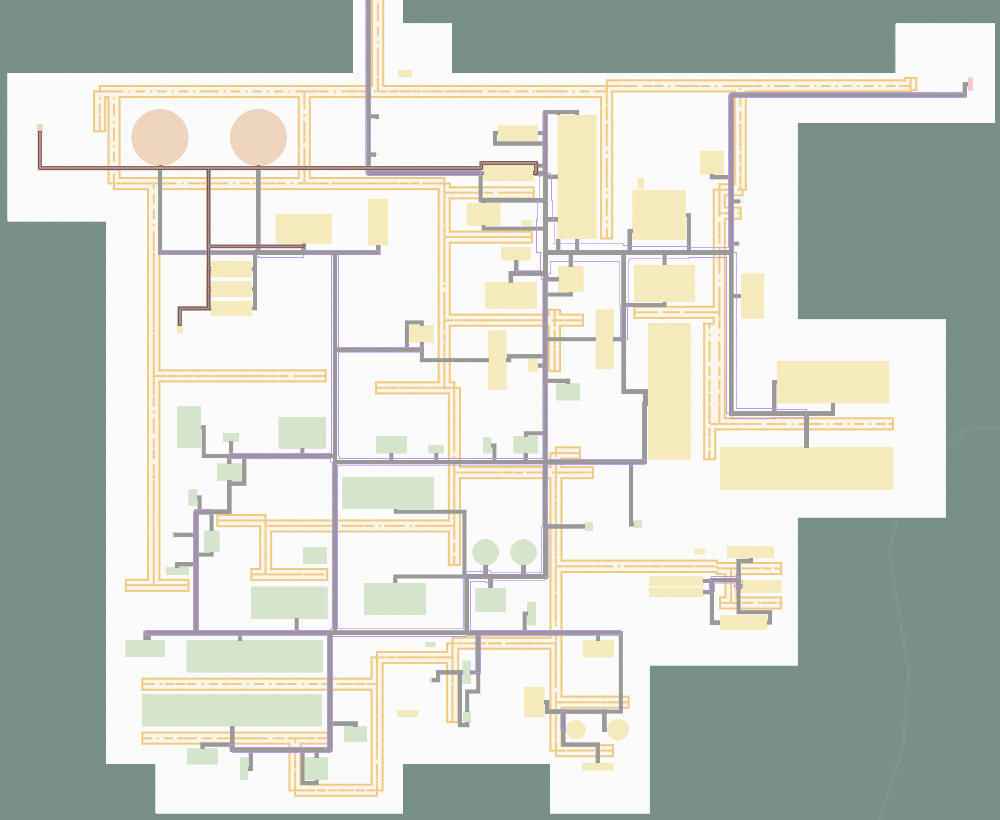
\includegraphics[width=0.8\textwidth]{images/problem/1}
    \end{center}
    \caption{Пример результата работы}
    \label{pic:problem__site-plan}
\end{wrapfigure}

\noindent В качестве результата работы системы получаем:
\begin{itemize}
    \item фигуру площадного объекта, содержащей заданные сооружения;
    \item местоположения сооружений;
    \item схемы технологических эстакад минимальной длины, соединяющей все сооружения, введенные пользователем;
    \item схему внутриплощадочных проездов;
    \item стоимость инженерной подготовки, коэффициента застройки территории и длины технологических связей;
    \item зоны распространения теплового потока;
    \item зоны распространения взрывной волны;
\end{itemize}

Система используется, как площадка
для исследований и демонстрации различных алгоритмических подходов для решения задачи,
так как полноценного решения математической задачи еще не существует.
Это ведет к тому, что существующая методика решения задачи может в одночасье стать неактуальной,
потому что найдется новая методика, которая будет давать более качественное решение.
Поэтому система должна быть очень гибкой, чтобы без больших затрат со стороны разработки вносить подобные изменения.


\textit{Целью данной работы} является анализ и обоснование применяемых технических решений в рамках реализации данной
системы.

Исходя из этой цели можно выделить следующие \textit{задачи}:
\begin{enumerate}
    \item проанализировать имеющиеся ресурсы для реализации системы,
    \item выбрать и обосновать технологический стек,
    \item cпроектировать архитектуру системы в целом и обосновать выбор компонентов системы,
    \item обосновать способ взаимодействия компонентов системы друг с другом.
\end{enumerate}


\subsection*{\large{Актуальность проблемы}}
\addcontentsline{toc}{subsection}{Актуальность проблемы}

Основной задачей системы является получения генерального
плана площадного объекта в автоматическом режиме
на основе заданного перечня сооружений,
технологических и инженерных связей, формы и размера участка местности,
доступного для застройки, а также требований нормативной документации.
Создание инструмента для аналитики и формирования генеральных планов
площадных объектов позволит снизить капитальные затраты
при строительстве промышленных объектов благодаря повышению качества проектирования.
Подобный инструмент позволит сравнить несколько различных вариантов планировок
одного промышленного объекта, чтобы впоследствии выбрать оптимальный по ряду критериев,
а также получить обоснование, почему выбранный вариант планировки действительно является оптимальным.


Данная задача является чрезвычайно сложной в алгоритмическом плане и не имеет готовых методик решения.
Для её решения требуется провести ряд научных исследований в области алгоритмов.
Процесс исследований напрямую связан с взаимодействием
с техническими экспертами в области проектирования генеральных планов.
